%%
%% User Guide
%%

%%%%%%%%%%%%%%%%%%%%%%%%%%%%%%%%%%%%%%%%%%%%%%%%%%%%%%%%%%%%%%%%%%%%%%%%%%%%%%%%
\chapter{User Guide}
%%%%%%%%%%%%%%%%%%%%%%%%%%%%%%%%%%%%%%%%%%%%%%%%%%%%%%%%%%%%%%%%%%%%%%%%%%%%%%%%


%%%%%%%%%%%%%%%%%%%%%%%%%%%%%%%%%%%%%%%%%%%%%%%%%%%%%%%%%%%%%%%%%%%%%%%%%%%%%%%%
\section{\qsimavr User Guide}
%%%%%%%%%%%%%%%%%%%%%%%%%%%%%%%%%%%%%%%%%%%%%%%%%%%%%%%%%%%%%%%%%%%%%%%%%%%%%%%%

Within this guide, we will assume the use of firmware compiled for the
\verb|atmega1280| with a frequency of 16 \ac{MHz}\footnote{
%
These are the default settings.
%
}. After starting \qsimavr, you are presented with a screen which should look
somewhat similar to figure \ref{fig:qsimavr}.

\begin{figure}[ht]
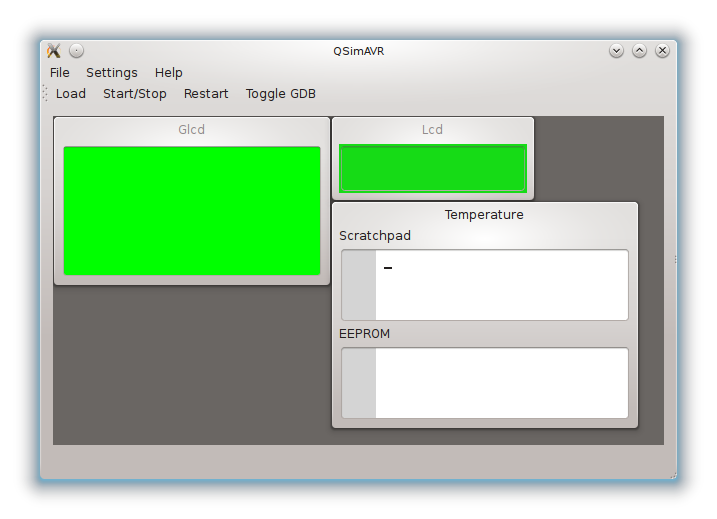
\includegraphics[width=\textwidth]{images/qsimavr}
\caption{\qsimavr}
\label{fig:qsimavr}
\end{figure}


%%%%%%%%%%%%%%%%%%%%%%%%%%%%%%%%%%%%%%%%%%%%%%%%%%%%%%%%%%%%%%%%%%%%%%%%%%%%%%%%
\section{Debugging with \simavr and \ac{GDB}} \label{section:debugging}
%%%%%%%%%%%%%%%%%%%%%%%%%%%%%%%%%%%%%%%%%%%%%%%%%%%%%%%%%%%%%%%%%%%%%%%%%%%%%%%%

% Mention how debugging with qsimavr is exactly the same.
